\graphicspath{{Chapter2/Figs/}}

\section{Model validation with simulated data} \label{section:mofa_simulated}

We used simulated data from the generative model to systematically test the technical capabilities of MOFA.

\subsection{Recovery of simulated factors}

First, we tested the ability of MOFA to recover simulated factors under varying number of views, features, factors and with different amounts of missing values.\\ 
For every simulation scenario we initialised a model with a high number of factors ($K=100$), and inactive factors were automatically dropped during model training by the ARD prior. In addition, to test the robustness under different random initialisations, 10 model instances were trained for every simulation scenario.\\
We observe that in most settings the model accurately recovers the correct number of factors (\Cref{fig:MOFA_learnK}). Exceptions occur when the dimensionality of the latent space is too large (more than 50 factors) or when an excessive amount of missing values (more than 80\%) is present in the data.

\begin{figure}[H]
	\centering 	
	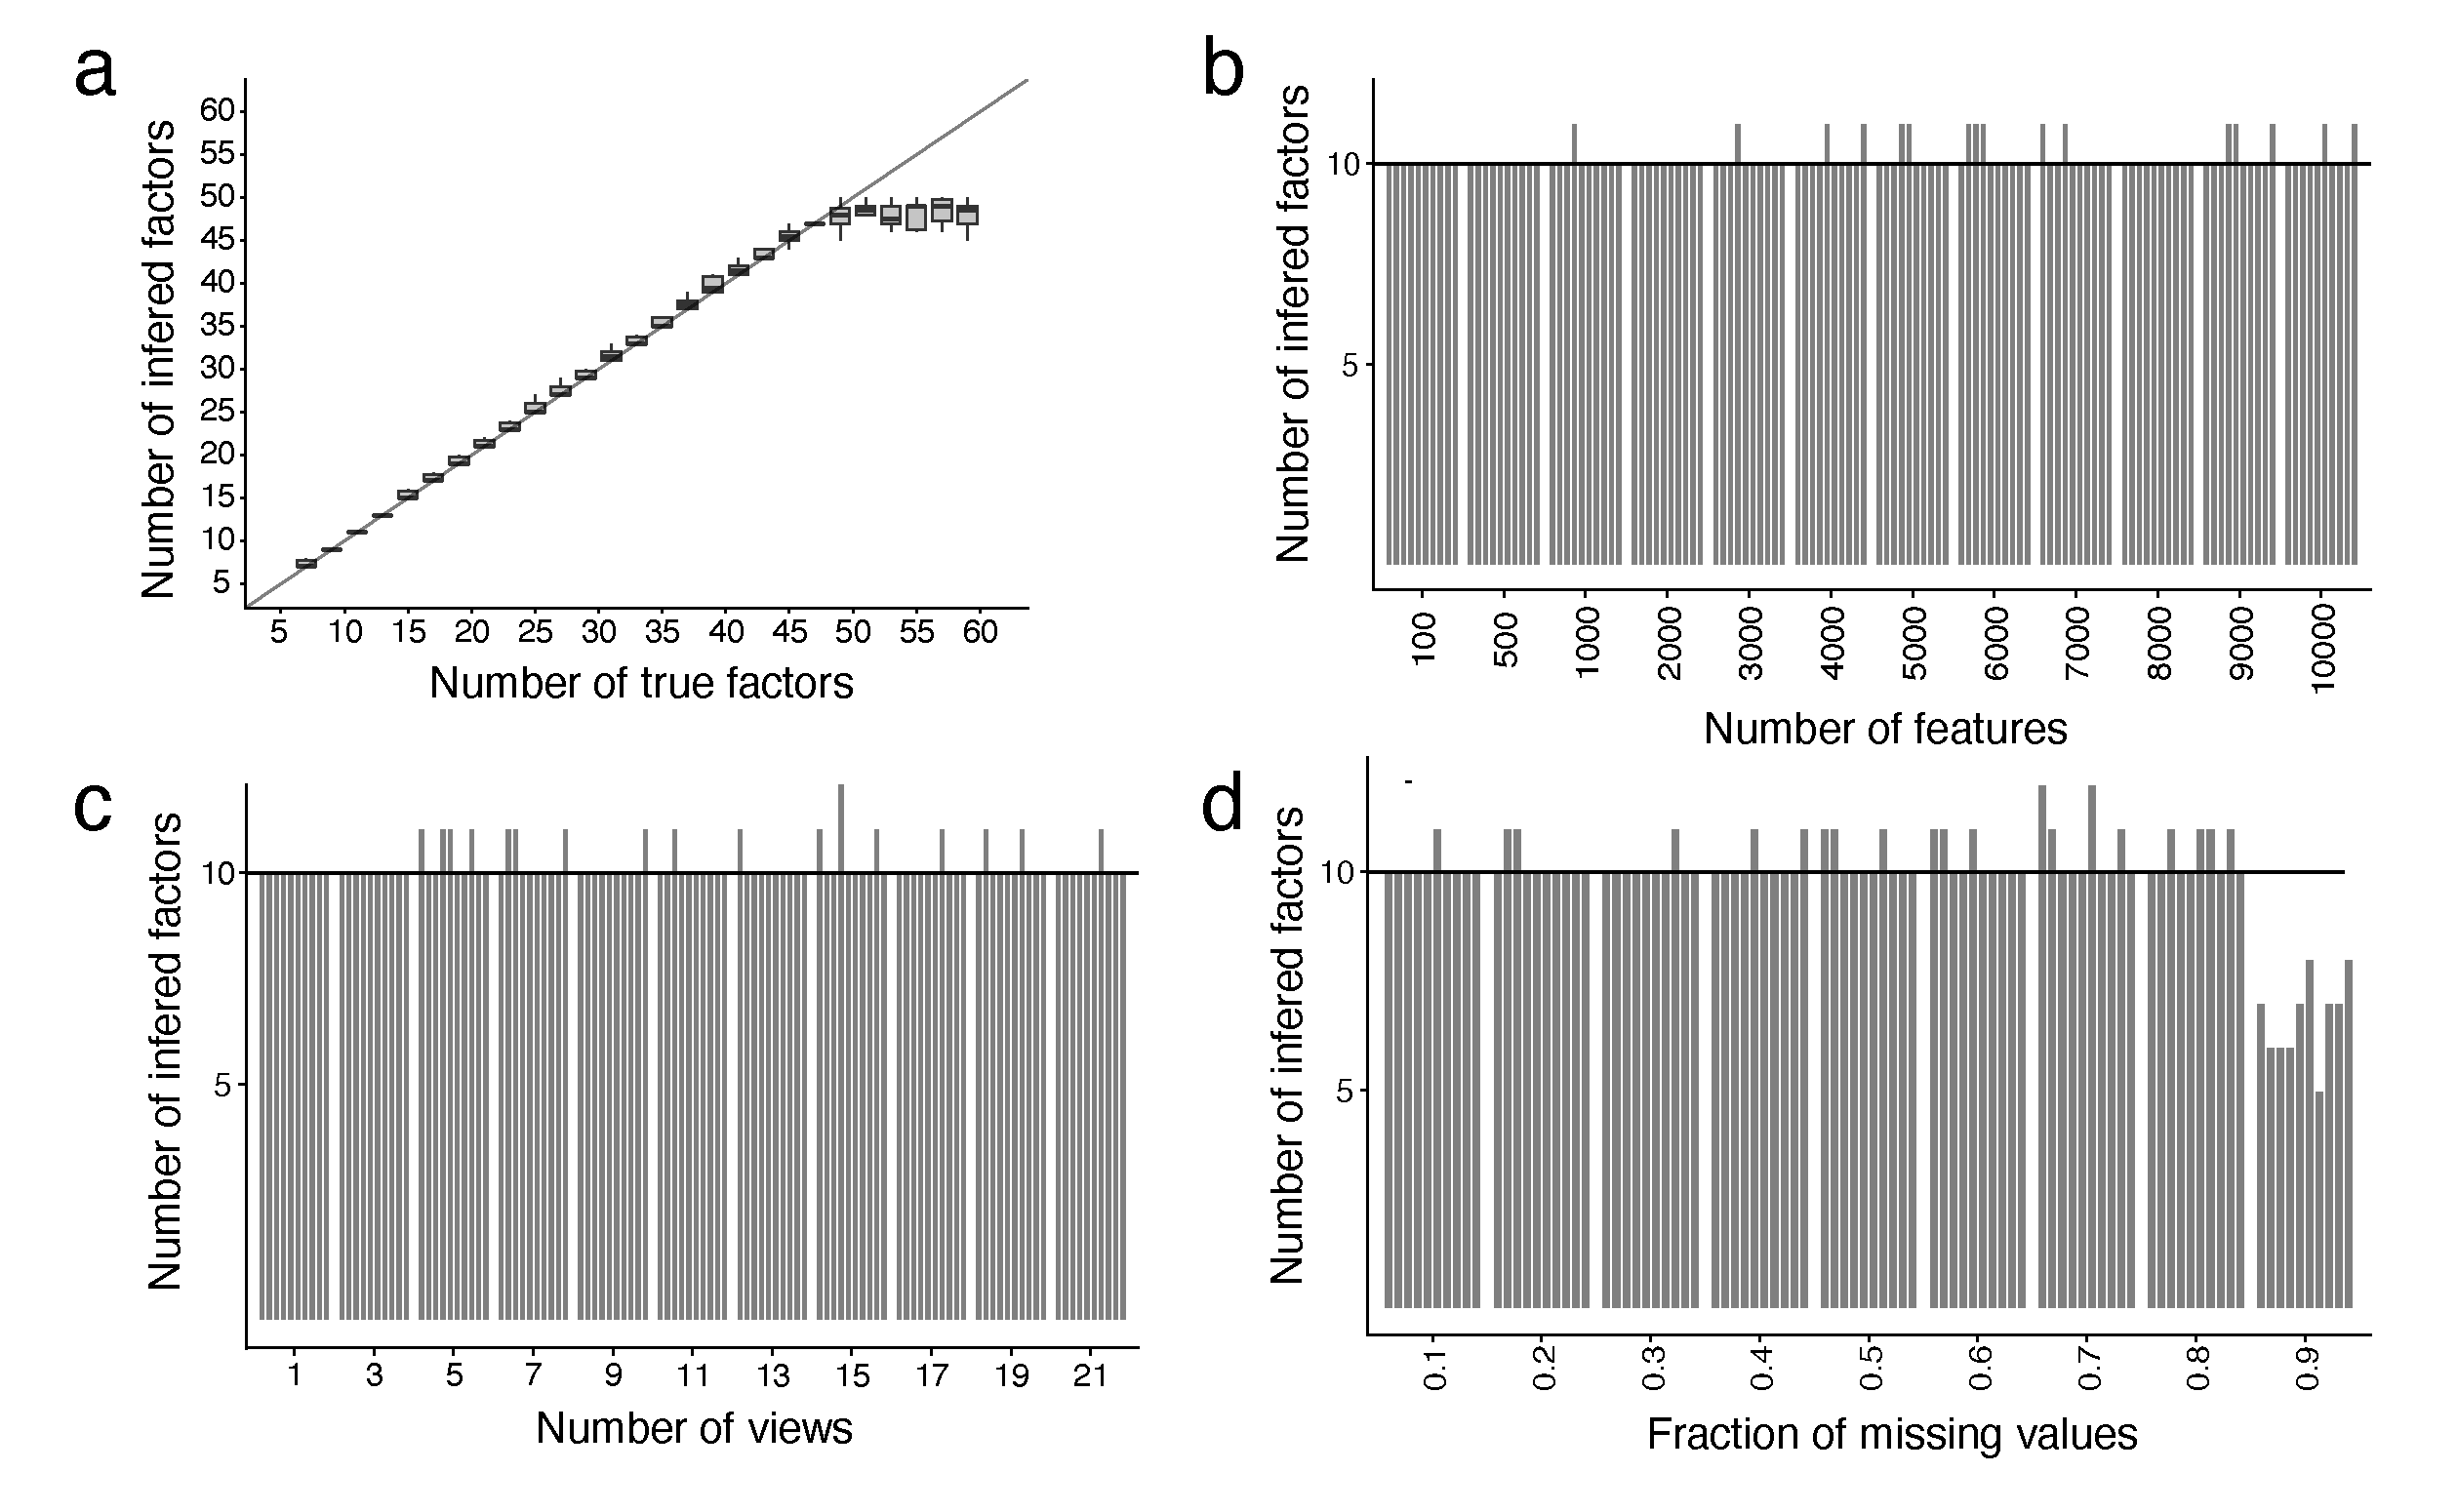
\includegraphics[width=0.9\textwidth]{MOFA_learnK}
	\caption{\textbf{Assessing the ability to recover simulated factors}.\\
	In all plots the y-axis displays the number of infered factors. (a) x-axis displays the number of true factors, and boxplots summarise the distribution across 10 model instances. For (b-d) the true number of factors was set to $K=10$ and each bar corresponds to a different model instance. (b) x-axis displays the number of features, (c) x-axis displays the number of views, (d) x-axis displays fraction of missing values. }
	\label{fig:MOFA_learnK}
\end{figure}

\subsubsection{View-wise sparsity on the weights}

One of the essential components that underlies MOFA is the use of an ARD prior aimed at disentangling the activity of factors across views (see \Cref{section_ard} and \Cref{mofa:model_description}).\\
We simulated data from the generative model were the factors were set to be active or inactive in specific views by sampling $\alpha_{k}^{m}$ from a discrete distribution with values $\{ 1, 1e3\}$. We compared the performance with a popular integrative clustering method (iCluster) that is also formulated as a latent variable model \cite{Mo2013}. In iCluster each factor shares the same sparsity constraint across all views, and hence the model is less accurate at detecting factors that show differential activity across different views:

\begin{figure}[H]
	\centering 	
	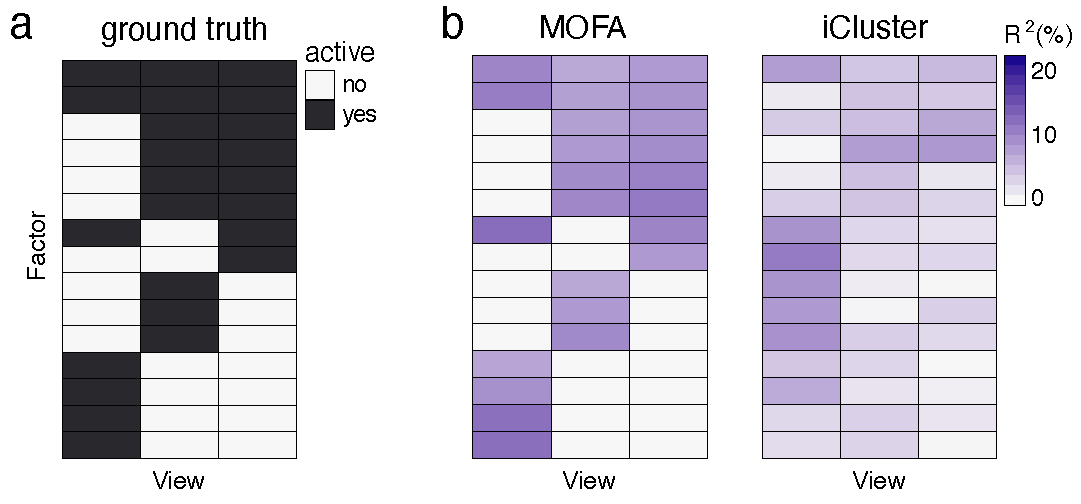
\includegraphics[width=0.9\textwidth]{MOFA_group_sparsity}
	\caption{\textbf{Evaluating the ability to recover differential factor activity across views}.\\
	(a) The true activity pattern, with factors sampled to display differential activity across views.
	(b) Percentage of variance explained for each factor in each view, for MOFA and iCluster \cite{Mo2013}.}
	\label{fig:MOFA_group_sparsity}
\end{figure}

\subsubsection{Feature-wise sparsity on the weights} \label{section:spike_slab}

In MOFA we implemented a spike-and-slab prior prior to enforce feature-wise sparsity on the weights with the aim of delivering a more interpretable solution (see \Cref{section:mofa_weights}).\\
To assess the effect of the spike-and-slab prior we trained a group of models with and without the spike-and-slab prior. Importantly, the model without spike-and-slab priors contains the ARD prior, which should provide some degree of regularisation. To compare both options to a non-sparse method, we also fit a Principal Component Analysis on the concatenated data set. As expected, we observe that the spike-and-slab prior induces more zero-inflated weights, although the ARD prior provided a moderate degree of regularisation. The PCA solution was notably more dense than both Bayesian models (\Cref{fig:MOFA_sparsity}).

\begin{figure}[H]
	\centering 	
	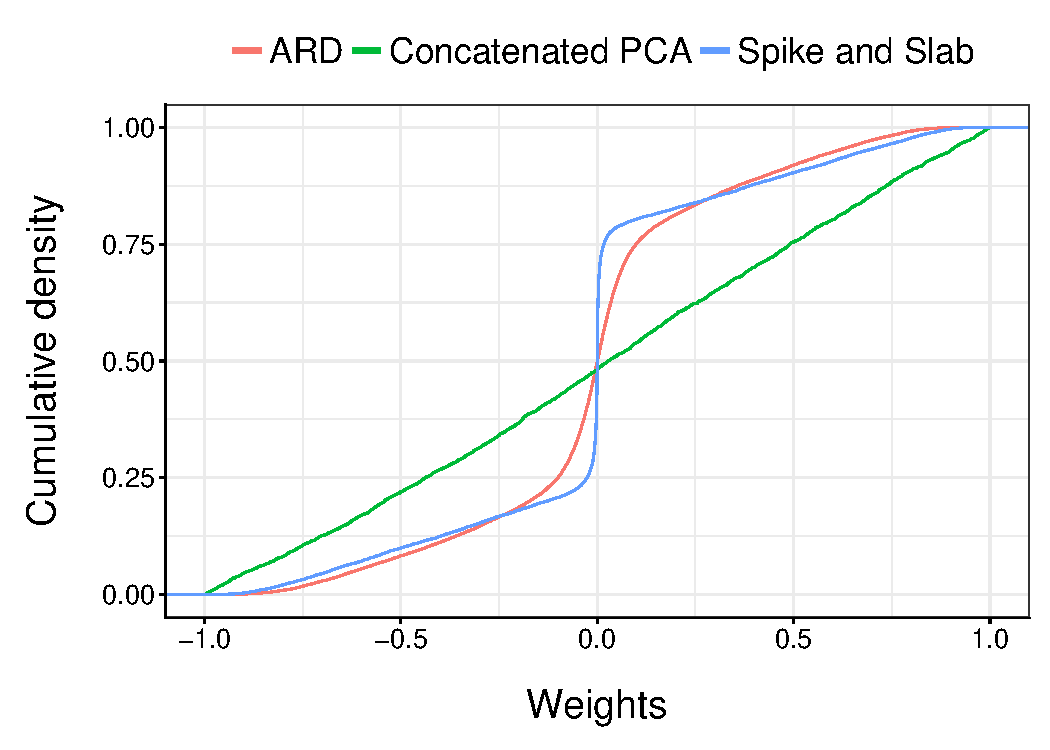
\includegraphics[width=0.7\textwidth]{MOFA_sparsity}
	\caption{\textbf{Assessing the sparsity priors on the weights}.\\ 
	The plot shows the empirical cumulative density function of the weights for an arbitrary factor in a single view. The weights were simulated with a sparsity level of $\theta_k^m=0.5$ (50\% of active features.)
	}
	\label{fig:MOFA_sparsity}
\end{figure}


\subsection{Non-Gaussian likelihoods}  \label{section:mofa_nongaussian_results}

A key improvement of MOFA with respect to previous methods is the use of non-Gaussian likelihoods to integrate data modalities with different types of readouts. In particular, as described in \Cref{section:mofa_ngaussian}, we implemented a Bernoulli likelihood to model binary data and a Poisson likelihood to model count data.\\
To validate both likelihood models, we simulated binary and count data using the generative model and we fit two sets of models for each data type: a group of models with a Gaussian likelihood and a group of models with a Bernoulli or Poisson likelihood, respectively.\\
Reassuringly, we observe that although the Gaussian likelihood is also able to recover the true number of factors, the models with the non-Gaussian likelihoods result in a better fit to the data:

\begin{figure}[H]
	\centering 	
	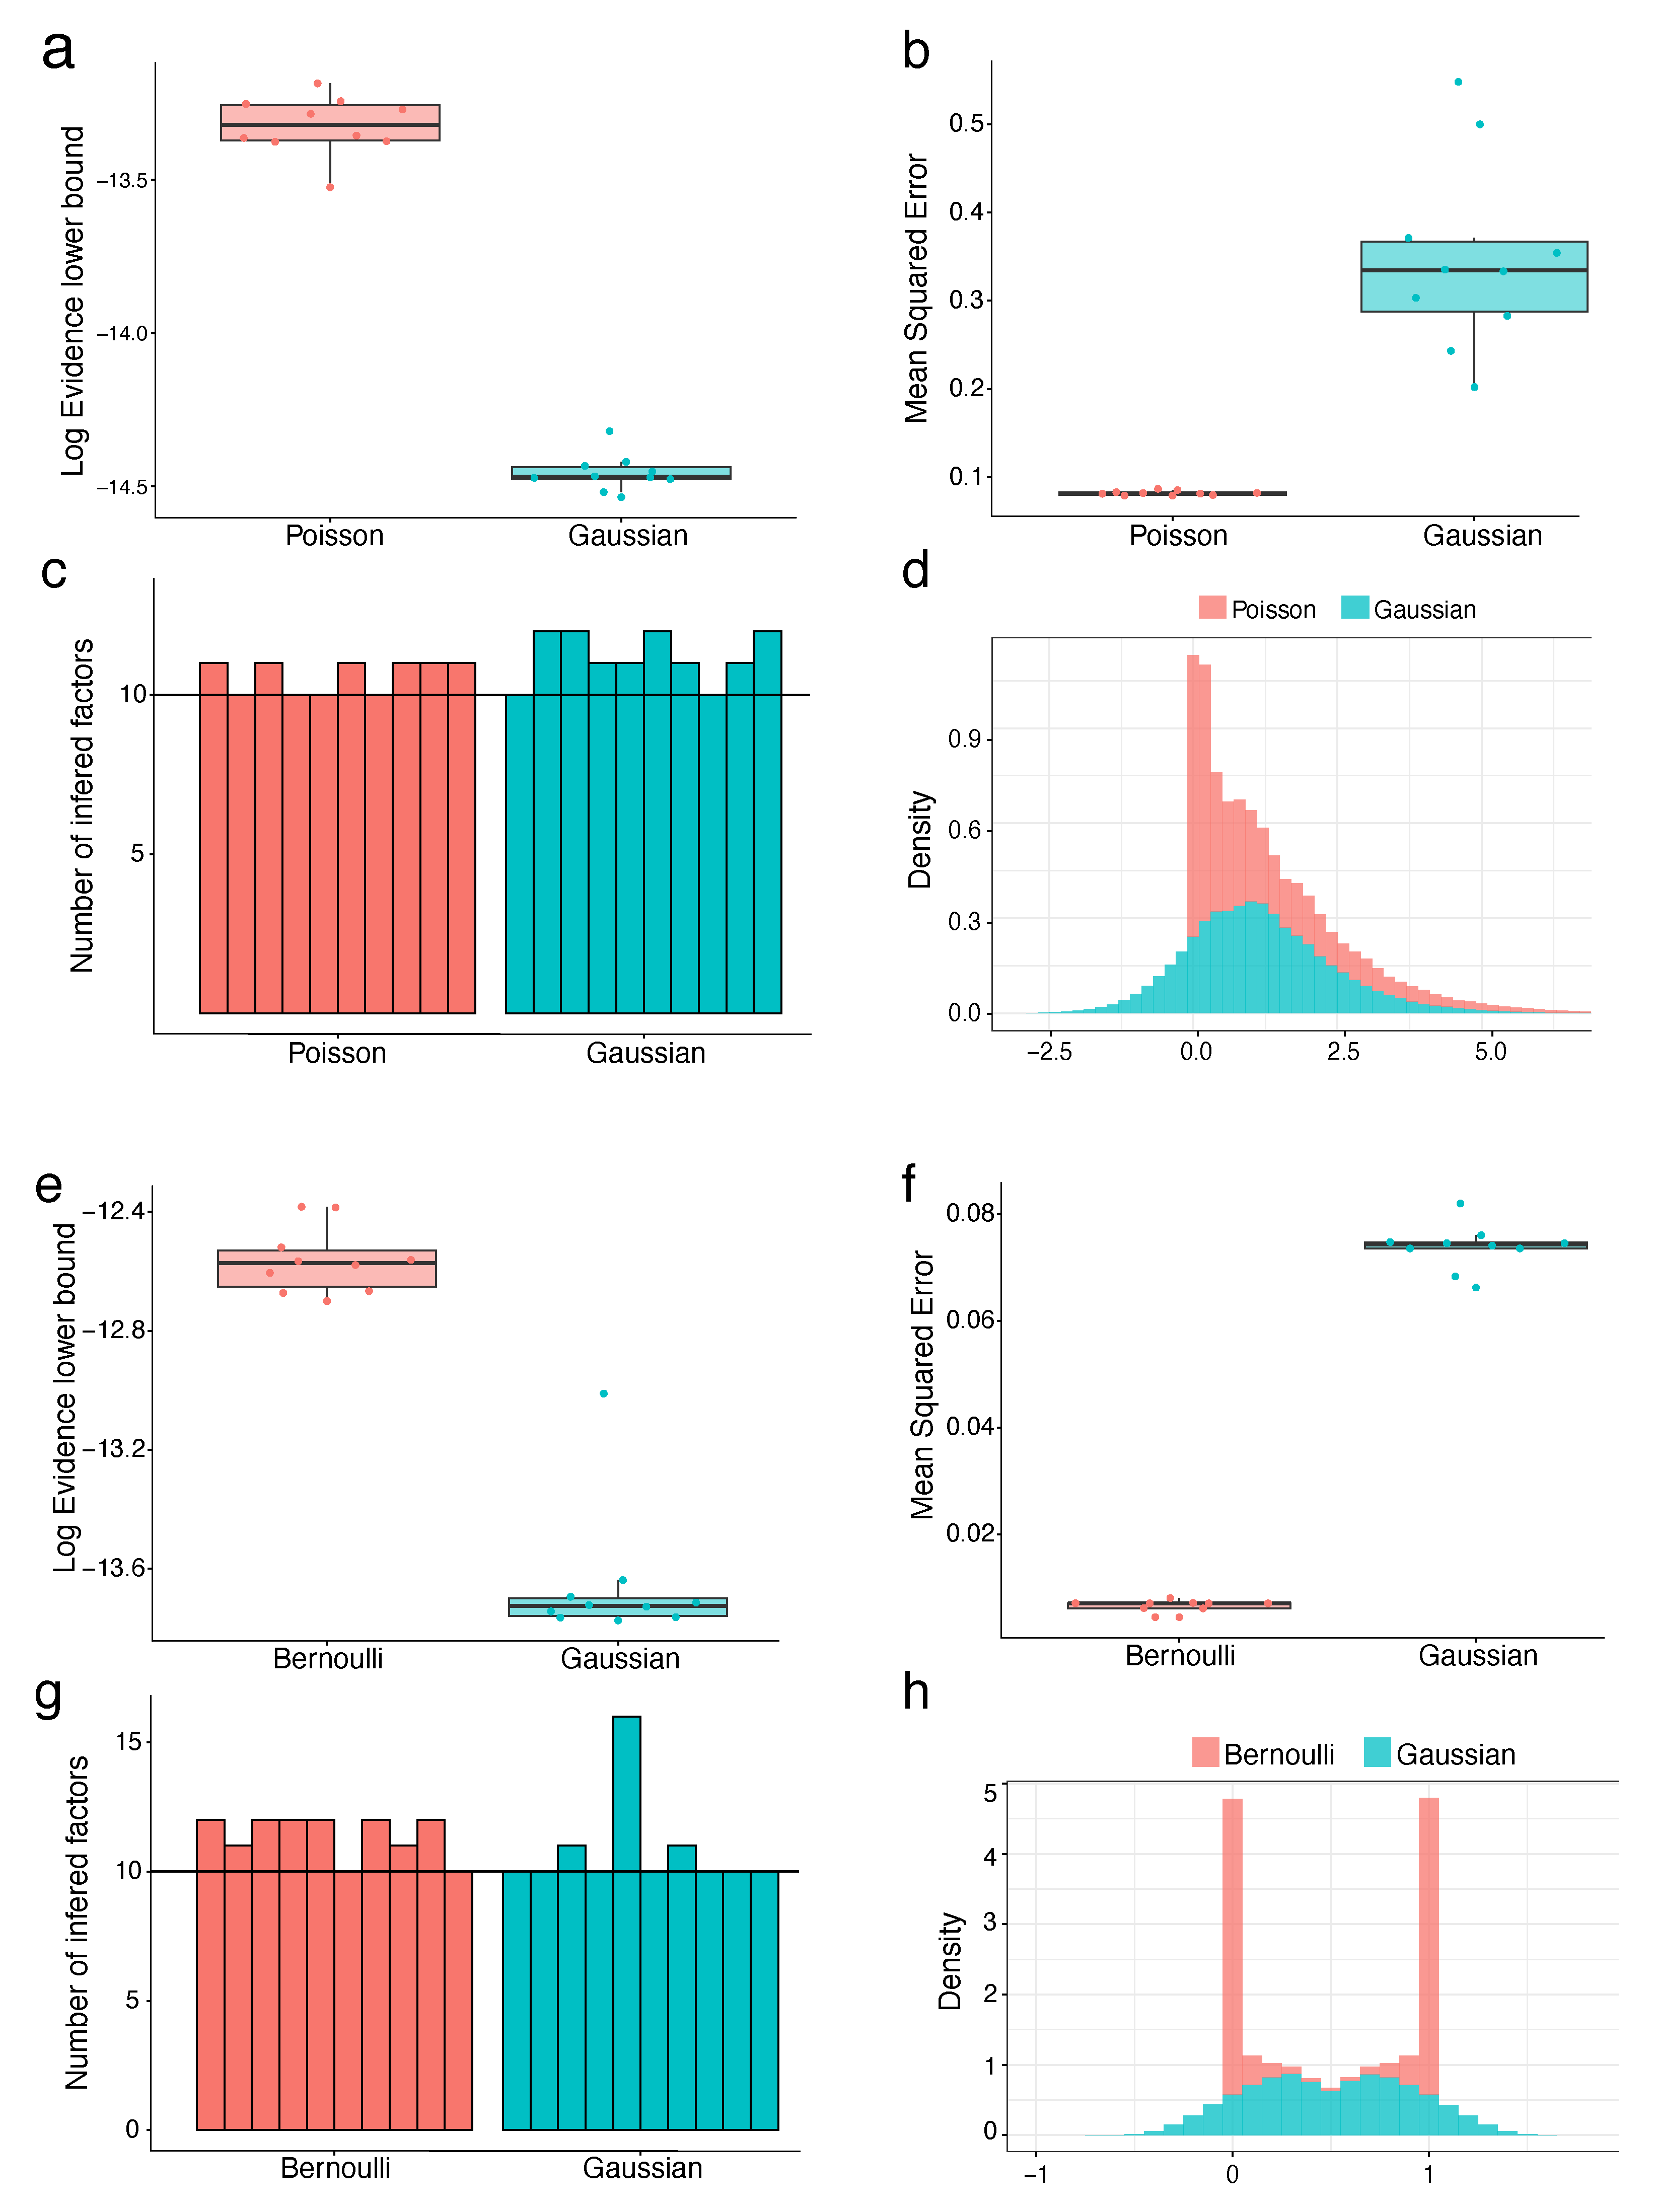
\includegraphics[width=0.8\textwidth]{MOFA_nongaussian}
	\caption{\textbf{Validation of the non-Gaussian likelihood models using simulated data}.\\
	(a-d) Comparison of Poisson and Gaussian likelihood models applied to count data.\\
	(e-h) Comparison of Bernoulli and Gaussian likelihood models applied to binary data.\\
	(a,e) The y-axis displays the ELBO for each model instance (x-axis). (b,f) The y-axis displays the mean reconstruction error for each model instance (x-axis). (c,g) The y-axis displays the number of estimated factrors for each model instance (x-axis). The horizontal dashed line marks the true number of factors $K=10$. (d,h) Distribution of reconstructed data. Plotted are the expected values of the inferred posterior distributions, not samples from the corresponding posteriors. This is why reconstructed measurements are continuous and not discrete.
	}
	\label{fig:MOFA_nongaussian}
\end{figure}


\subsection{Scalability}

Finally, we evaluated the scalability of the model when varying each of its dimensions independently, and we compared the speed with an implementation of GFA that uses Gibbs Sampling \cite{Leppaaho2017} and the popular Cluster+\cite{Mo2013}, which adopts a maximum-likelihood approach with grid search to optimise the hyperparameters. Overall, we observe that MOFA scales linear with respect to all dimensions and is significantly faster than any of the three evaluated techniques (\Cref{fig:MOFA_scalability}).

\begin{figure}[H]
	\centering 	
	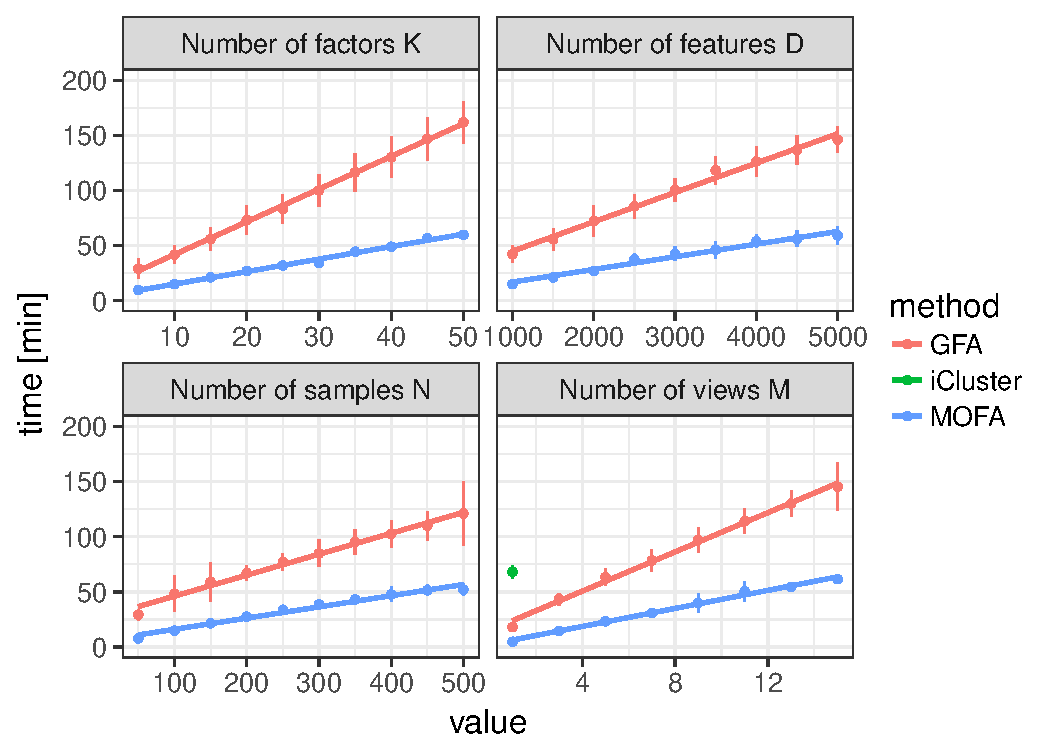
\includegraphics[width=0.75\textwidth]{MOFA_scalability}
	\caption{\textbf{Evaluation of scalability in MOFA}.\\
	Shown is the time required for convergence (y-axis, in minutes). The x-axis displays the value of the dimension that was tested, either number of factors ($K$), number of features ($D$), number of samples ($N$) and number of views ($M$). Baseline parameters were $M=3, K=10, D=1000, N=100$. Each line represents a different model, GFA (red), MOFA (blue) and iCluster (green). Default convergence criteria where used for all methods. Each dot displays the average time across 10 trials with error bars denoting the standard deviation. iCluster is only shown for one value as all other settings required more than 200min for convergence.
	}
	\label{fig:MOFA_scalability}
\end{figure}

As a real application showcase, the training on the CLL cohort that is described below (\Cref{fig:MOFA_CLL_overview}) required 25 minutes using MOFA, 34 hours with GFA and 5-6 days with iCluster.

% \subsection{Class imbalance}  \label{section:class_imbalance}
% TO-DO.
%The objective function (the evidence lower bound, ELBO) does not weight the different data modalities according to the number of features. Hence, in general the larger the number of features
%Having said this, we find the model to be very robust to differences in the dimensionality of the feature space.


\newpage

\section{Application to a cohort of Chronic Lymphocytic Leukaemia patients} \label{section:mofa_cll}

Personalised medicine is an attractive field for the use of multi-omics, as dissecting heterogeneity across patients is a major challenge in complex diseases, and requires data integration from multiple biological layers \cite{Chen2013,Costello2014,Alyass2015}.

To demonstrate the potential of the method, we applied MOFA to a publicly available study of 200 patient samples of Chronic Lymphocytic Leukaemia (CLL) profiled for somatic mutations, RNA expression, DNA methylation and \textit{ex vivo} drug responses \cite{Dietrich2018}, all of them being bulk samples. We selected this data set for three main reasons: (1) The complex missing data structure, with nearly 40\% samples having incomplete assays (\Cref{fig:MOFA_CLL_overview}). As described in \Cref{section:mofa_missing_values}, the inference framework implemented in MOFA should cope with large amounts of missing values, including missing assays. (2) After data processing, three assays had continuous observations whereas for the somatic mutations the observations were binary. As described in \Cref{section:mofa_ngaussian}, MOFA can combine different likelihood models. (3) The existence of clinical covariates provide an excellent test to evaluate whether the MOFA factors can capture the molecular variation that underlies clinically-relevant phenotypes.

\subsection{Data overview and processing}

Data processing and normalisation is essential for the model to work and it requires a few considerations. First, in the case of count-based assays such as RNA-seq one needs to remove differences in library size between samples. If not done correctly, the signal in the data will be dominated by this (undesired) source of variation, and more subtle heterogeneity will be harder to identify. Similarly, batch effects and other undesired technical sources of variation should be regressed out \textit{a priori}, although this was not the case for this particular data set. Second, feature selection must be performed by selecting highly variable features. A proper feature selection will increase the signal-to-noise-ratio, it will simplify model selection and it will speed up the training procedure.  Finally, as discussed above, the total number of features can influence the contribution of a data modality to the latent space. To mitigate this problem it is recommended to keep the number of features per view within the same order of magnitude, when possible.

Here we proceed to briefly describe the different data modalities and outline the basic data processing steps that we performed before applying MOFA:
\begin{itemize}
	\item \textbf{RNA expression} was profiled using bulk RNA-seq. Genes with low counts were filtered out and the data was subsequently normalized using DESeq2 \cite{Love2014}. Feature selection was performed by considering the top 5,000 most variable genes.
	\item \textbf{DNA methylation} was profiled using Illumina 450K arrays. We converted the beta-values to M-values, as it has better statistical properties when modelled with a Gaussian distribution \cite{Du2010}. Feature selection was performed by considering the top 1\% most variable CpG sites. 
	\item \textbf{\textit{Ex vivo} Drug response} was screened using the ATP-based CellTiter-Glo assay. Briefly, the asay includes a panel of 62 drugs at 5 different concentrations each, for a total of 310 measurements. The readout is a number proportional to the fraction of viable cells in culture based on quantitation of the ATP present, which signals the presence of metabolically active cells.
	\item \textbf{Somatic mutations} were profiled using a combination of targeted and whole exome sequencing. Feature selection was performed by considering only mutations that were present in at least three samples, which resulted in a total of 69 mutations.
\end{itemize}

% For more details on the data generation steps we refer the reader to \cite{Dietrich2018}.

\subsection{Model overview}

In this data set, MOFA recovered $K=10$ factors, each one explaining a minimum of 3\% of variance in at least one assay. Interestingly, MOFA detects factors which are shared across several data modalities (Factors 1 and 2, sorted by variance explained). Some factors capture sources of covariation between two data modalities (Factor 3 and 5, active in the RNA expression and drug response). In addition, some factors capture variation that is unique to a single data modality (Factor 4, active in the RNA expression data).\\
All together, the 10 MOFA factors explained 41\% of variance in the drug response data, 38\% in the mRNA expression, 24\% in the DNA methylation and 24\% in somatic mutations.

\begin{figure}[H]
	\centering 	
	\includegraphics[width=1.0\textwidth]{MOFA_CLL_overview}
	\caption{\textbf{Application of MOFA to a study of chronic lymphocytic leukaemia. Model overview.}\\
	(a) Data overview. Assays are shown in different rows ($D$ = number of features) and samples ($N$) in columns, with missing samples shown using grey bars. Notice that some samples are missing entire assays.\\
	(b) Variance explained (\%) by each Factor in each assay.\\
	(c) Total variance explained (\%) for each assay by all factors.
	}
	\label{fig:MOFA_CLL_overview}
\end{figure}

The first two factors are the most interesting from a molecular perspective, as they capture a phenotypic effect that is manifested across all molecular layers, from the genome to the transcriptome and ultimately in the drug response assay.\\
To annotate Factors 1 and 2 we proceeded to visualise the feature weights, starting by the (binary) somatic mutation data, as it is the simplest data modality to interpret. Inspection of the top weights revealed that Factor 1 was associated with the mutation status of the immunoglobulin heavy-chain variable (IGHV) region, while Factor 2 was aligned with trisomy of chromosome 12 (\Cref{fig:MOFA_CLL_factors12}).\\
Remarkably, in a completely unsupervised fashion, MOFA recovered the two most important clinical markers in CLL as the two major axes of molecular disease heterogeneity \cite{Fabbri2016,Bulian2017,Crombie2017}.

Next, we visualised the samples in the latent space spanned by Factors 1 and 2. A scatterplot based on these factors shows a clear separation of patients by their IGHV status on the first Factor and presence or absence of trisomy 12 on the second Factor (\Cref{fig:MOFA_CLL_factors12}). Interestingly, 24 patients lacked IGHV status measurements (see grey crosses) due to quality control filtering in the DNA sequencing assay. Nonetheless, MOFA is able to pool information from the other molecular layers to map those samples to the latent space, and could be classified to the corresponding molecular subgroup.

\begin{figure}[H]
	\centering 	
	\includegraphics[width=1.0\textwidth]{MOFA_CLL_factors12}
	\caption{\textbf{Visualisation of the genetic signature underlying Factor 1 and 2}\\
	(a) Absolute weights of the top features of Factors 1 and 2 in the Mutations data.
	(b) Visualization of samples using Factors 1 and 2. The colours denote the IGHV status of the tumours; symbol shape and colour tone indicate chromosome 12 trisomy status.
	}
	\label{fig:MOFA_CLL_factors12}
\end{figure}

IGHV status is currently the most important prognostic marker in CLL and has routinely been used to distinguish between two distinct subtypes of the disease\cite{Fabbri2016}. Molecularly, it is a surrogate of the level of activation of the B-cell receptor, which is in turn related to the differentiation state of the tumoral cells. Multiple studies have associated mutated IGHV with a better resposne to chemoimmunotherapy, whereas unmutated IGHV patients have a worse prognosis \cite{Fabbri2016,Bulian2017,Crombie2017}.\\
In clinical practice, the IGHV status has been considered binary. Our results suggest that this is a fairly good approximation, but a more complex structure with at least three groups or a potential underlying continuum (\Cref{fig:MOFA_CLL_factors12,fig:MOFA_CLL_Factor1}), as also suggested in \cite{Queiros2015}.

% \subsection{Detection of outlier samples}

% Interestingly, there is some discrepancy between the IGHV status predicted by MOFA and the IGHV status reported in the clinical data. Out the 200 patients, MOFA classifies 176 in accordance with the clinical label, it classifies 12 patients that lacked the clinical marker and it re-classifies 12 patients to the opposite group.\\
% To validate the MOFA-based classification, we proceeded to inspect the molecular data in more detail.

% sample-to-sample correlation matrices for the individual layers suggest that for 3 of the cases where the inferred factor disagrees with the clinical label, the molecular data supports the predicted label. The other 9 cases showed intermediate molecular sgnatures now well captured by the binary classification.
% %Based on these results, we hypothesize that a multi-omics approach based on several molecular signatures could be a more precise and robust approach to predict clinical phenotypes than the use of single features such as mutations or expression of marker genes.

% \begin{figure}[H]
% 	\centering 	
% 	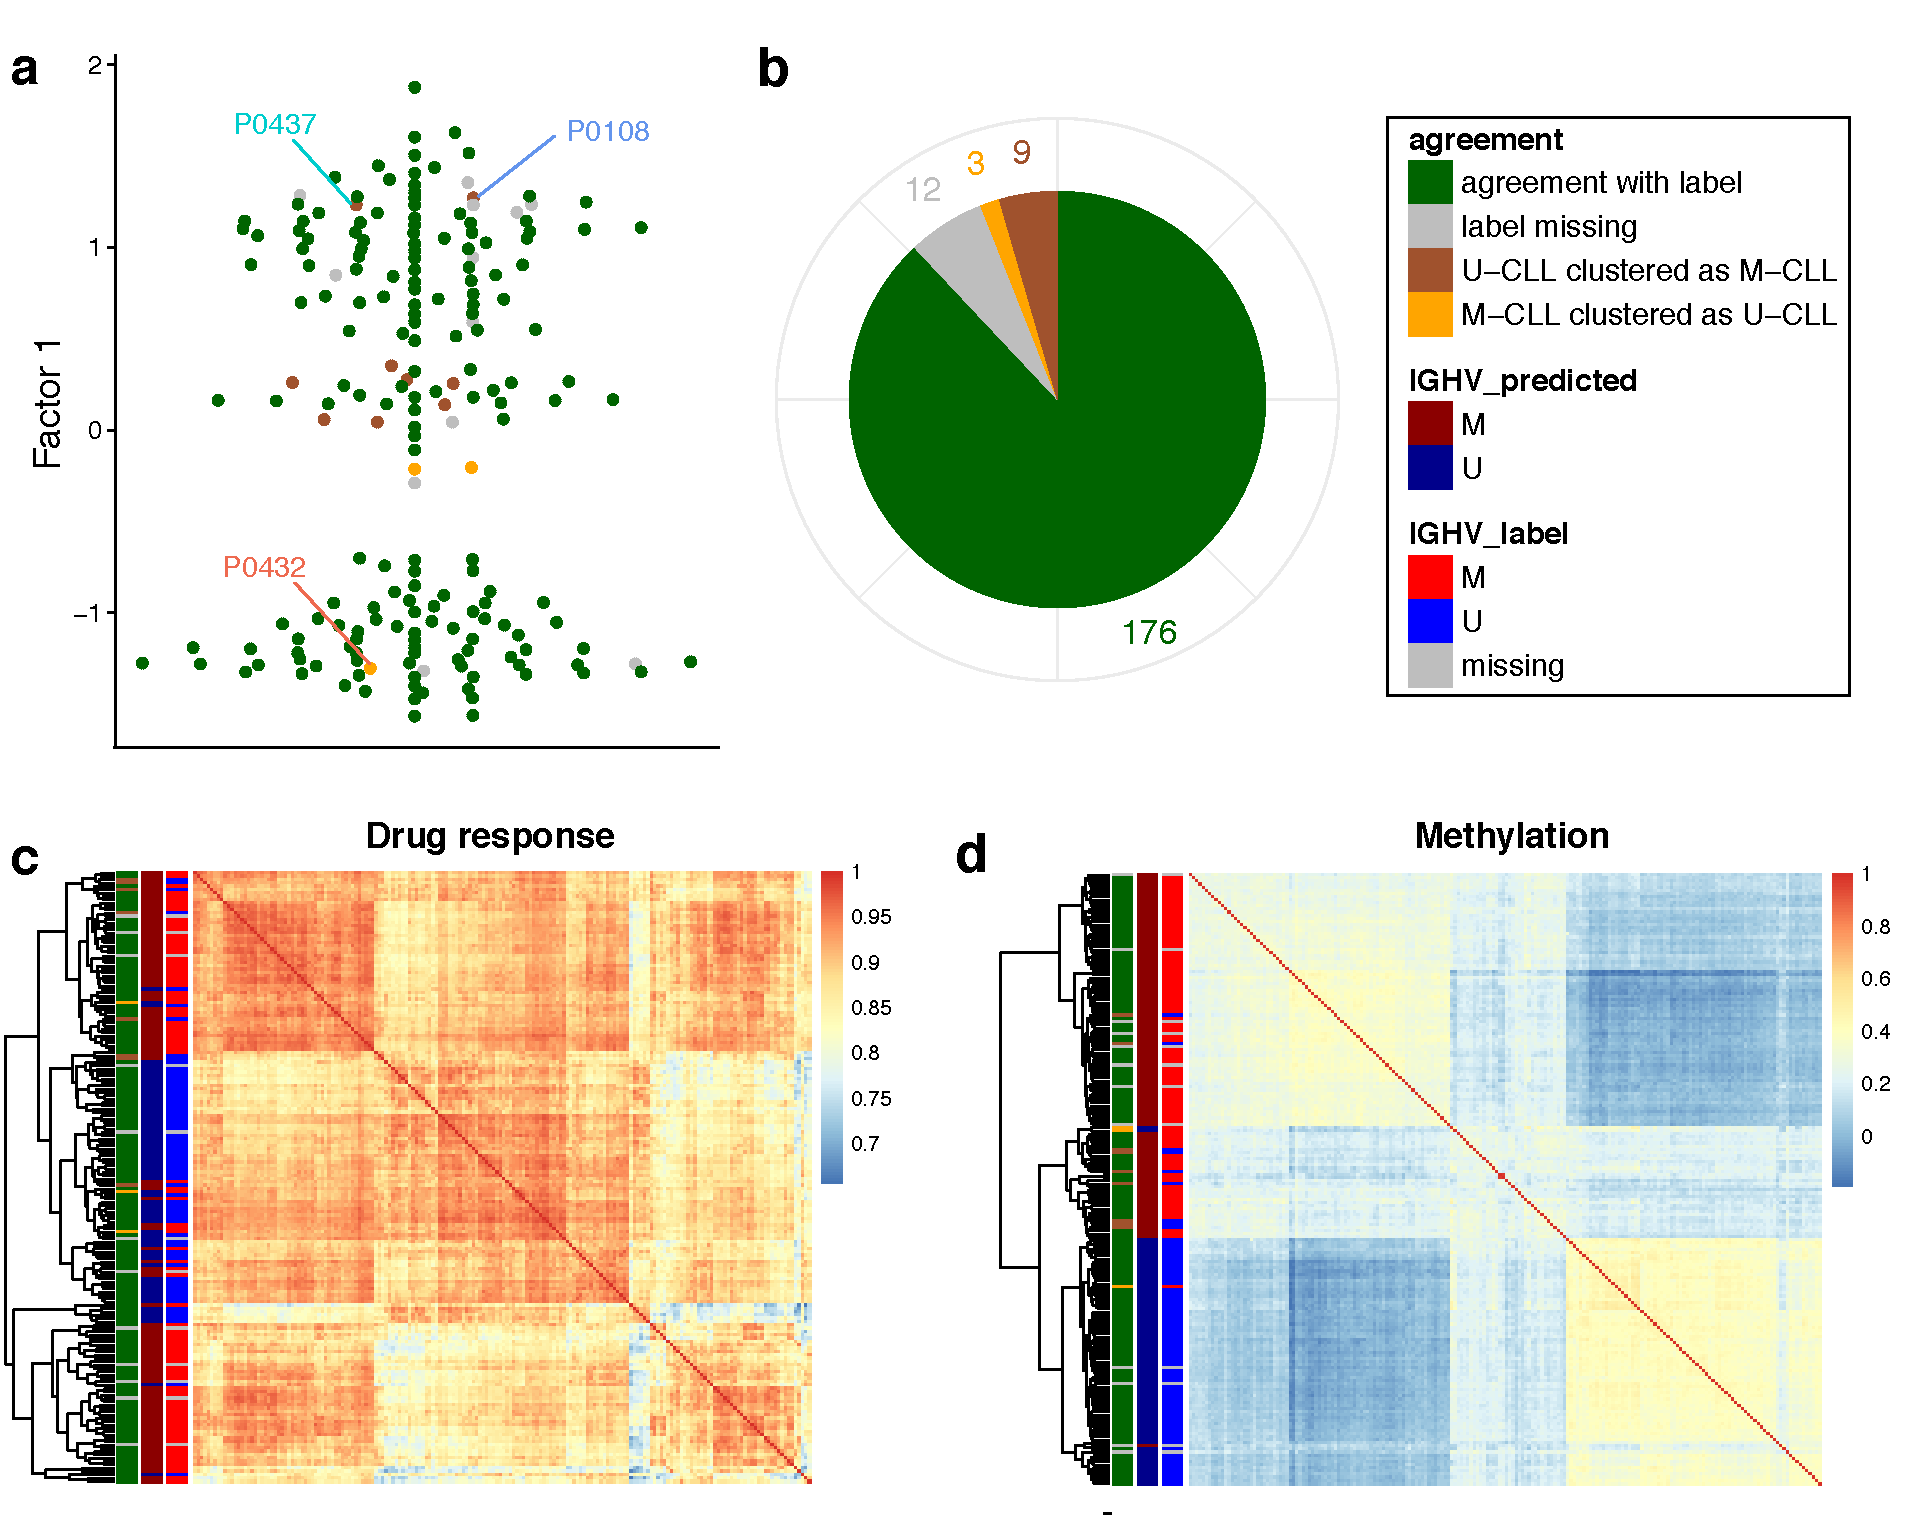
\includegraphics[width=1.0\textwidth]{MOFA_IGHV_outlier}
% 	\caption{XX}
% 	\label{fig:MOFA_IGHV_outlier}
% \end{figure}

\subsection{Molecular characterisation of Factor 1}
% \tabularnewline

An important step in the MOFA pipeline is the characterisation of the molecular signatures underlying each Factor. I will demonstrate this for Factor 1, although a similar strategy can be applied to Factor 2.

On the RNA expression, inspection of the top weights pinpoint genes that have been previously associated to IGHV status, some of which have been proposed as clinical markers\cite{Vasconcelos2005,Morabito2015}. Heatmaps of the RNA expression levels for these genes reveals clear differences between samples when ordered according to the Factor 1 values.

On the drug response data the weights highlight kinase inhibitors targeting the B-cell receptor pathway. Splitting the patients into three groups based on k-means clustering shows clear separation in the drug response curves.

% Copied
\begin{figure}[H]
	\centering 	
	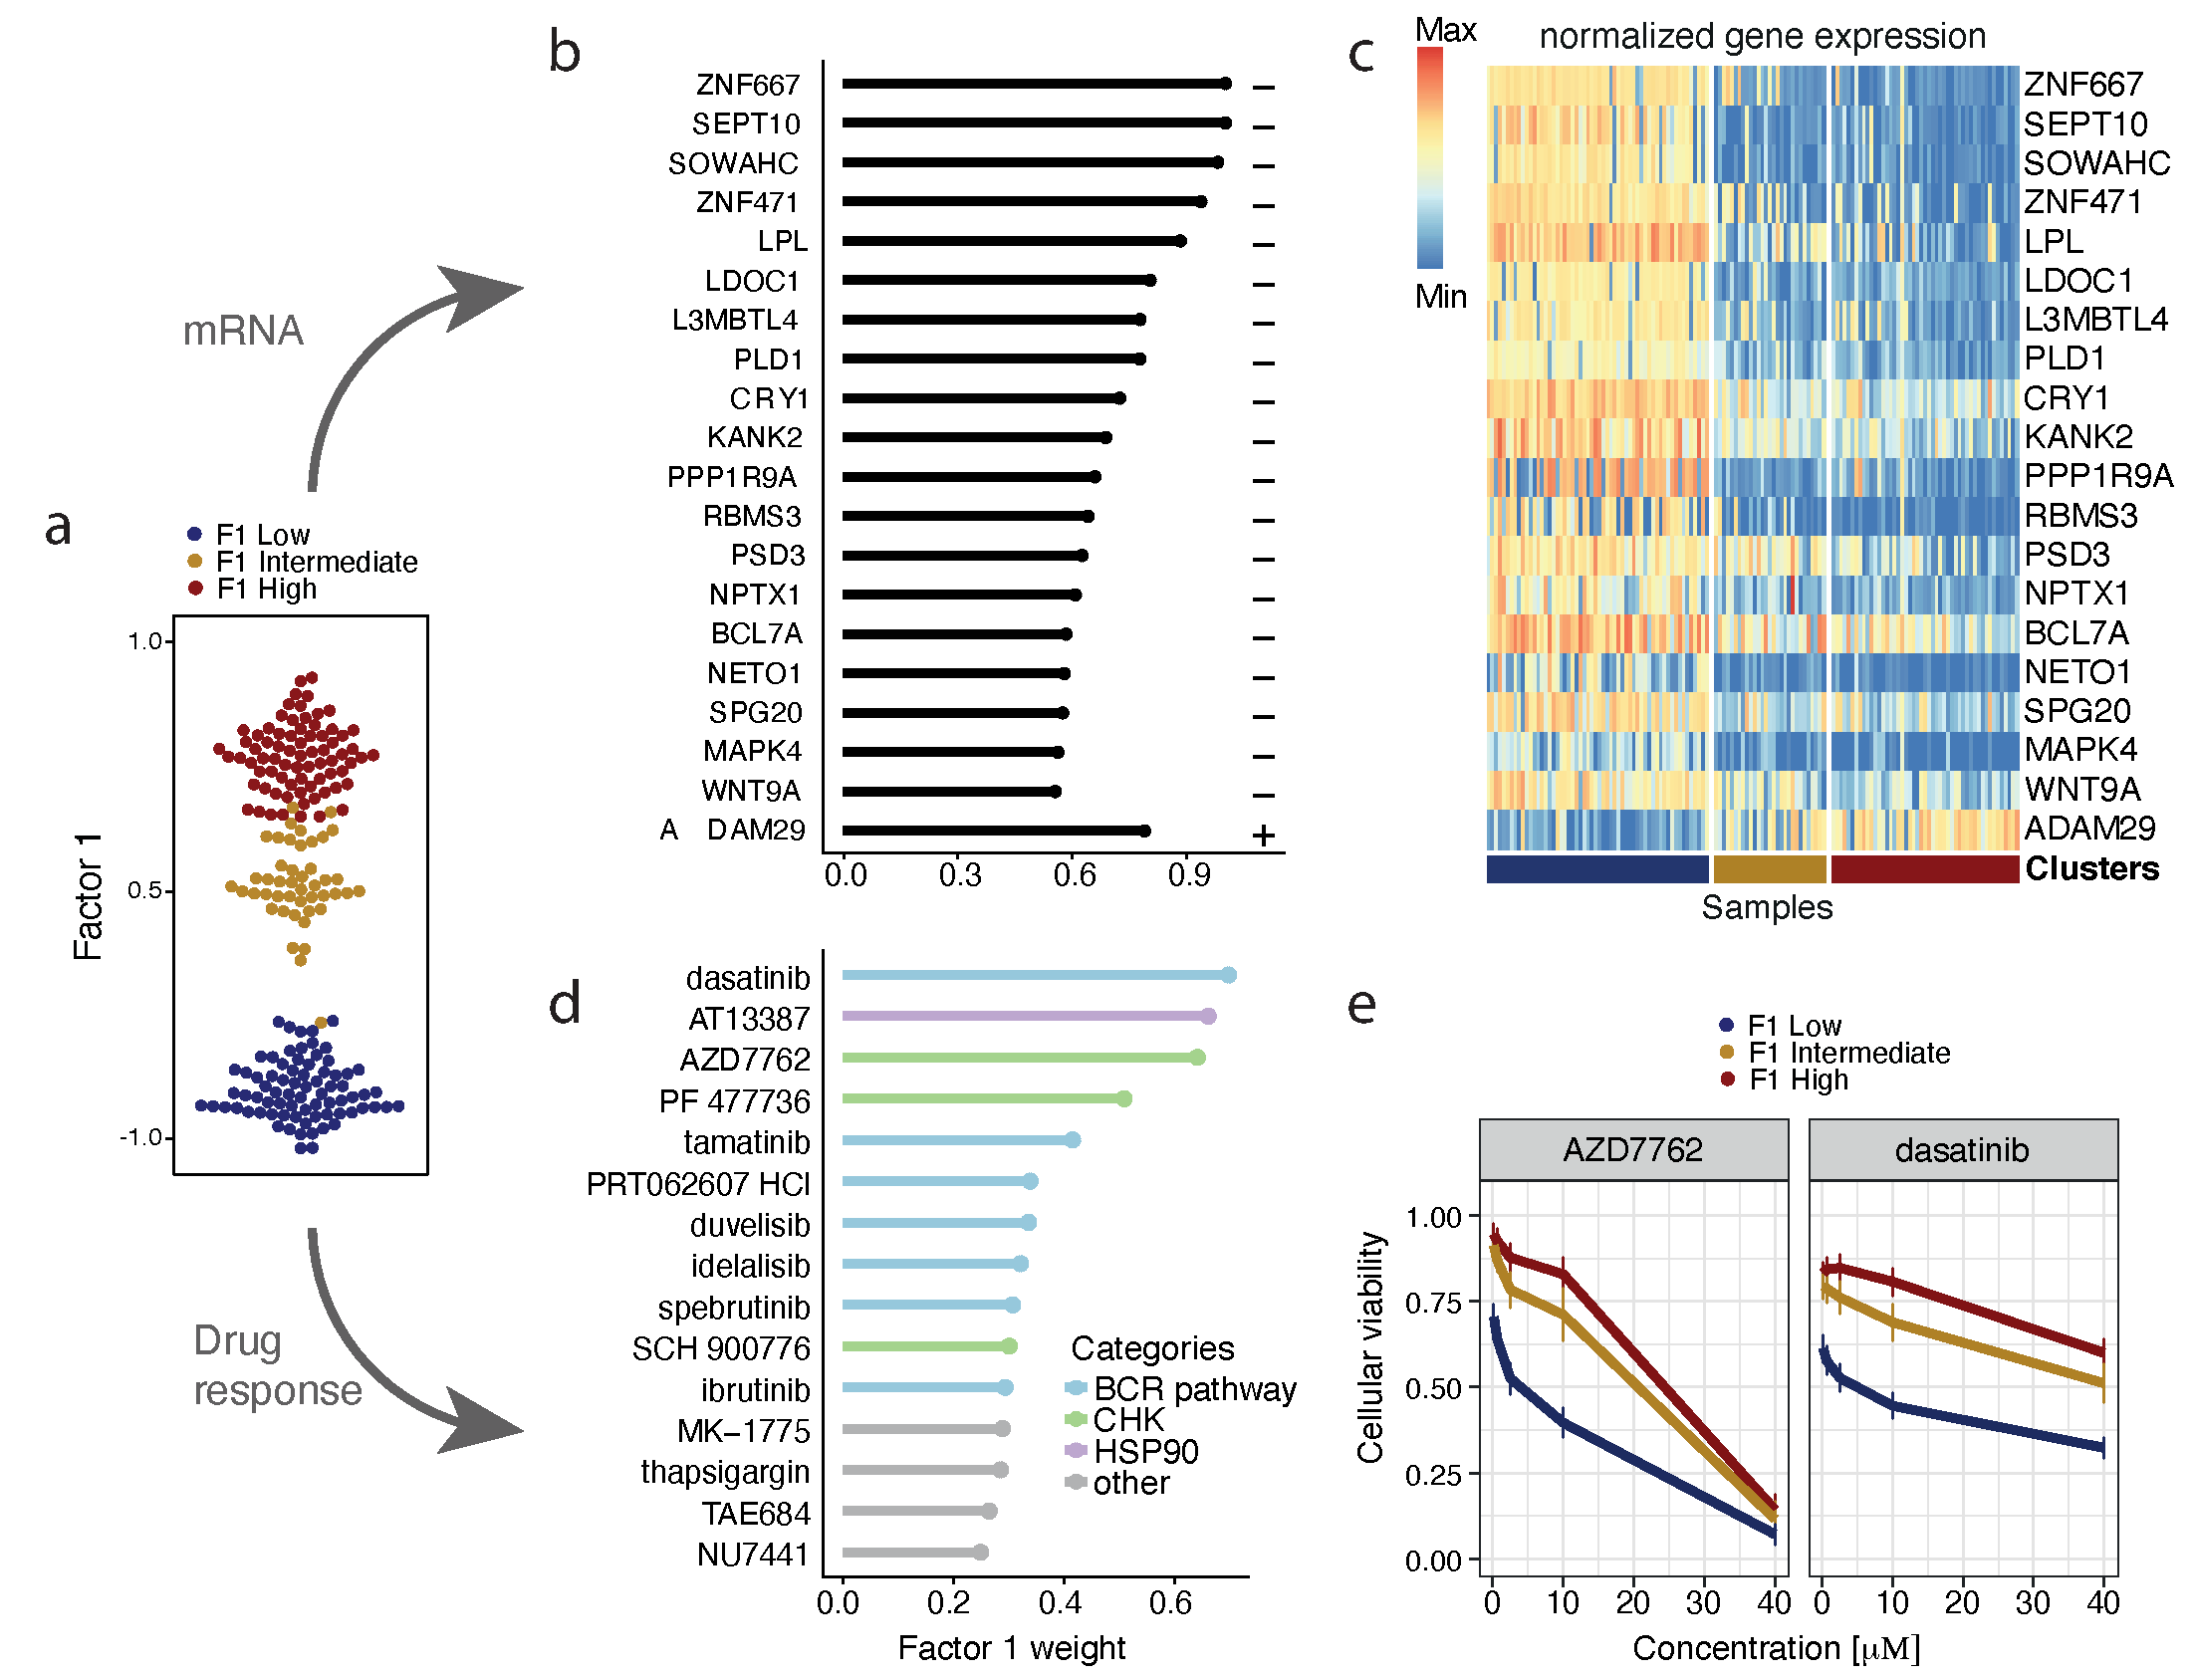
\includegraphics[width=0.90\textwidth]{MOFA_CLL_Factor1}
	\caption{
	\textbf{Characterization of MOFA Factor 1 as IGHV status.}\\
	(a) Beeswarm plot with Factor 1 values for each sample with colours corresponding to three groups found by 3-means clustering with low factor values (LZ), intermediate factor values (IZ) and high factor values (HZ).\\
	(b) Absolute weights for the genes with the largest absolute weights in the mRNA data. Plus or minus symbols on the right indicate the sign of the loading. Genes highlighted in orange were previously described as prognostic markers in CLL and associated with IGHV status (Vasconcelos et al, 2005; Maloum et al, 2009; Trojani et al, 2012; Morabito et al, 2015; Plesingerova et al, 2017).\\
	(c) Heatmap of gene expression values for genes with the largest weights as in (b).\\
	(d) Absolute weights of the drugs with the largest weights, annotated by target category.\\
	(e) Drug response curves for two of the drugs with top weights, stratified by the clusters as in (a).
	}
	\label{fig:MOFA_CLL_Factor1}
\end{figure}

\subsection{Molecular characterisation of other factors}

Despite their clinical importance, Factor 1 (IGHV status) and Factor 2 (chr12 trisomy) they explain less than 20\% variability in each data modality, suggesting the existence of more subtle sources of variation. As an example, we will also characterise Factor 5, which explains 2\% of the variance in the mRNA and 6\% of variance in the drug response.\\
As mentioned in \Cref{mofa:downstream}, instead of exploring the feature weights individually, factors can be annotated using gene set annotations. This procedure is particularly appealing for RNA expression data, as a rich amount of resources exist that have categorised genes into ontologies in terms of biological pathways, molecular function and cellular components  \cite{Fabregat2015,Ashburner2000}.

Briefly, the idea is to aggregate the weights using prior information to obtain a single statistic for each gene set, which can be tested against a competitive null hypothesis. Inspired from \cite{Frost2015}, in MOFA we implemented several scoring schemes and a variety of parametric and unparametric statistical tests. By default we use the weights as feature statistics and the average difference in the weight values as the feature set statistic. P-values are then obtained per feature set and factor via a simple t-test.

Gene Set Enrichment Analysis on the RNA weights using the Reactome annotations \cite{Fabregat2015} reveals that Factor 2 is strongly enriched for oxidative stress and senescence pathways. Inspection of the top features highlights the importance of heat shock proteins (HSPs), a group of proteins that are essential for protein stability which are up-regulated upon stress conditions like high temperatures, pH shift or oxidative stress. Importantly, HSPs can be elevated in tumour cells and potentially contribute to prolonged tumour cell survival\cite{Dempsey2010}. In agreement with the findings from the mRNA view, the drugs with largest weights on Factor 5 belong to clinical categories associated with stress response, such as target reactive oxygen species and DNA damage response (\Cref{fig:MOFA_CLL_Factor5})

\begin{figure}[H]
	\centering 	
	\includegraphics[width=0.95\textwidth]{MOFA_CLL_Factor5}
	\caption{
	\textbf{Characterization of Factor 5 in the CLL cohort as oxidative stress response.}\\
	(a) Beeswarm  plot of Factor 5. Colours denote the expression of TNF, an inflammatory stress marker that is present among the top mRNA weights.\\
	(b) Gene set enrichment analysis for the top Reactome pathways. Displayed are the top pathways with the strongest enrichment in the mRNA weights.\\
	(c) Heatmap of mRNA expression values for representative genes among the top  weights. Samples are ordered by their Factor 5 values.\\
	(d) Weights for the top drugs, annotated by target category.\\
	(e) Heatmap of drug response values for the top three drugs.
	}
	\label{fig:MOFA_CLL_Factor5}
\end{figure}


\subsection{Prediction of clinical outcomes}

We conjectured that the integration of multiple molecular layers could allow an improved prediction of the patients' clinical outcome.\\
To evaluate the utility of the MOFA factors as predictors of clinical outcomes we fit Cox regression models \cite{Cox1972} using the patients' time to next treatment (TTT) as a response variable. Two types of analysis were performed: a univariate analysis where each Factor was independently associated with TTT, and a multivariate analysis where the combination of all factors were used to predict TTT (\Cref{fig:MOFA_CLL_Cox}).\\
In the univariate Cox models, we observe  that Factor 1 (IGHV status), Factor 7 (associated with chemo-immunotherapy treatment prior to sample collection) and Factor 8 (enriched for Wnt signalling) were significant predictors of TTT. Accordingly, when splitting patients into binary groups based on the corresponding Factor values, we observe clear differences in the survival curves.\\
In the multivariate Cox model, MOFA (Harrell's C-Index C=0.78) outperformed all other input settings, including PCA on single-omic data (C=0.68-0.72), individual genetic markers (C=0.66) as well PCA applied to the concatenated data matrix (C=0.74).

%As predictors, we included the top 10 principal components calculated on the data for each single view, a concatenated data set ('all') as well as the 10 MOFA factors. Missing values in a view were set to the feature-wise mean. 

% Caption copied
\begin{figure}[H]
	\centering 	
	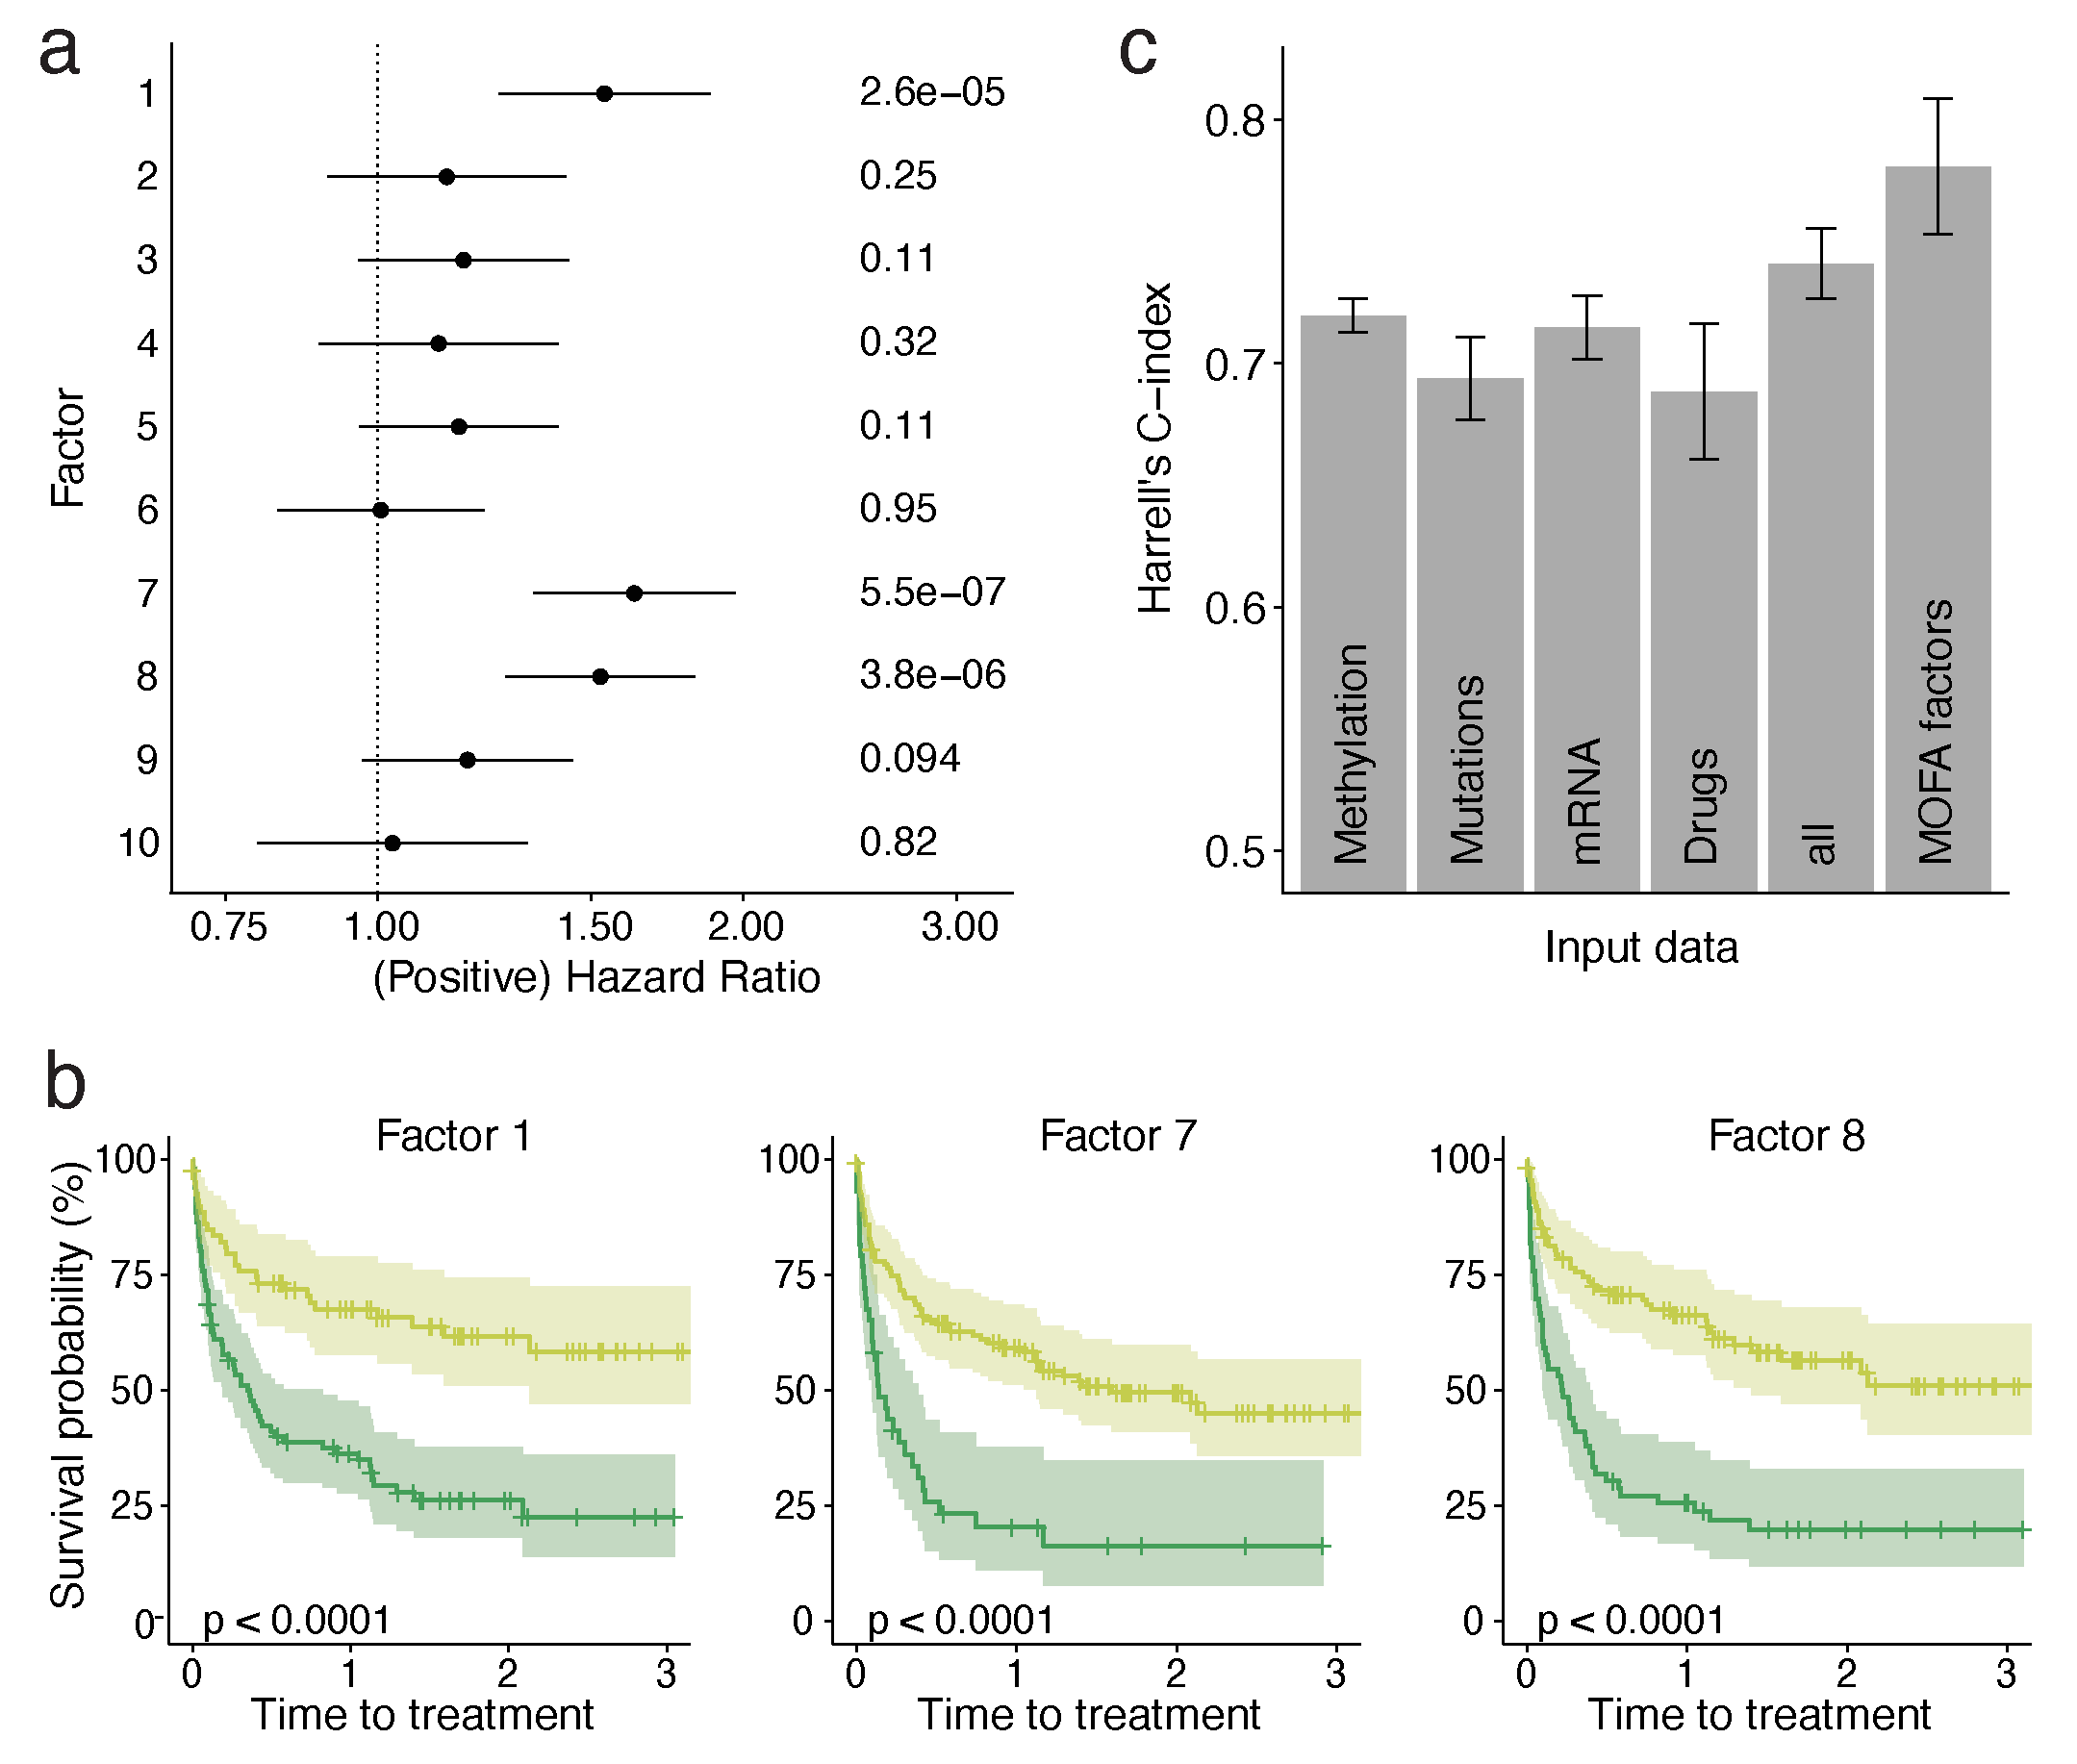
\includegraphics[width=0.9\textwidth]{MOFA_CLL_Cox}
	\caption{
	\textbf{Association analysis between MOFA factors and clinical putcome.}\\
	(a) Association of MOFA factors to time to next treatment using a univariate Cox regression with N = 174 samples (96 of which are uncensored cases) and p-values based on the Wald statistic. Error bars denote 95\% confidence intervals. Numbers on the right denote p-values for each predictor.\\
	(b) Kaplan-Meier plots measuring time to next treatment for the individual MOFA factors. The cut-points on each factor were chosen using maximally selected rank statistics, and p-values were calculated using a log-rank test on the resulting groups.\\
	(c) Prediction accuracy of time to treatment for N = 174 patients using multivariate Cox regression trained with the 10 MOFA factors, as well using the first 10 principal components applied to single data modalities and the full data set. Shown are average values of Harrell's C-index from fivefold cross-validation. Error bars denote standard error of the mean.
	}
	\label{fig:MOFA_CLL_Cox}
\end{figure}


\subsection{Imputation of missing values}

A promising application of MOFA is the imputation of missing values, including the potential to impute of entire assays.\\
The principle of imputation in MOFA follows the same logic as simulating from the generative model: if the factors and weights are known, the input data can be reconstructed by a simple matrix multiplication:
\[
	\hat{\bfY} = \E[\bfZ] \E[\bfW]^T
\]
where $\E[\bfZ]$ and $\E[\bfW]$ denote the expected values of the variational distributions for the factors and the weights, respectively. Notice that, when using the expectations of the posterior distributions, the noise $\epsilon$ (\Cref{mofa_master_equation}) has a mean of zero and does not contribute to the predictions.\\
The equation above results in point estimates, but it ignores the uncertainity on $\bfZ$ and $\bfW$. Instead of relying in point estimates, one could adopt a more Bayesian approach and calculate the posterior predictive distribution by propagating the uncertainity \cite{Gelman2013}. Nonetheless, due to the nature of the optimisation problem in variational inference, the variance of the posterior distributions can be underestimated (see \Cref{section:expectation_propagation}). In addition, this would be substantially more complex to implement and would result in a significant increase in computational complexity, hence we did not implement this strategy.

To assess the imputation performance, we trained MOFA models using a data set of complete measurements (a total of N=121 samples) after masking parts of the drug response measurements. In a first experiment, we masked values at random, and in a second experiment we masked the entire drug response measurements. We compared the imputation accuracy of MOFA to some established imputation strategies, including imputation by feature-wise mean, SoftImpute \cite{Mazumder2010}, and a k-nearest neighbour method \cite{Troyanskaya2001}. For both imputation tasks, MOFA consistently yielded more accurate predictions, albeit the differences are less pronounced in the imputation of full assays, a significantly more challenging task.\\

\begin{figure}[H]
	\centering 	
	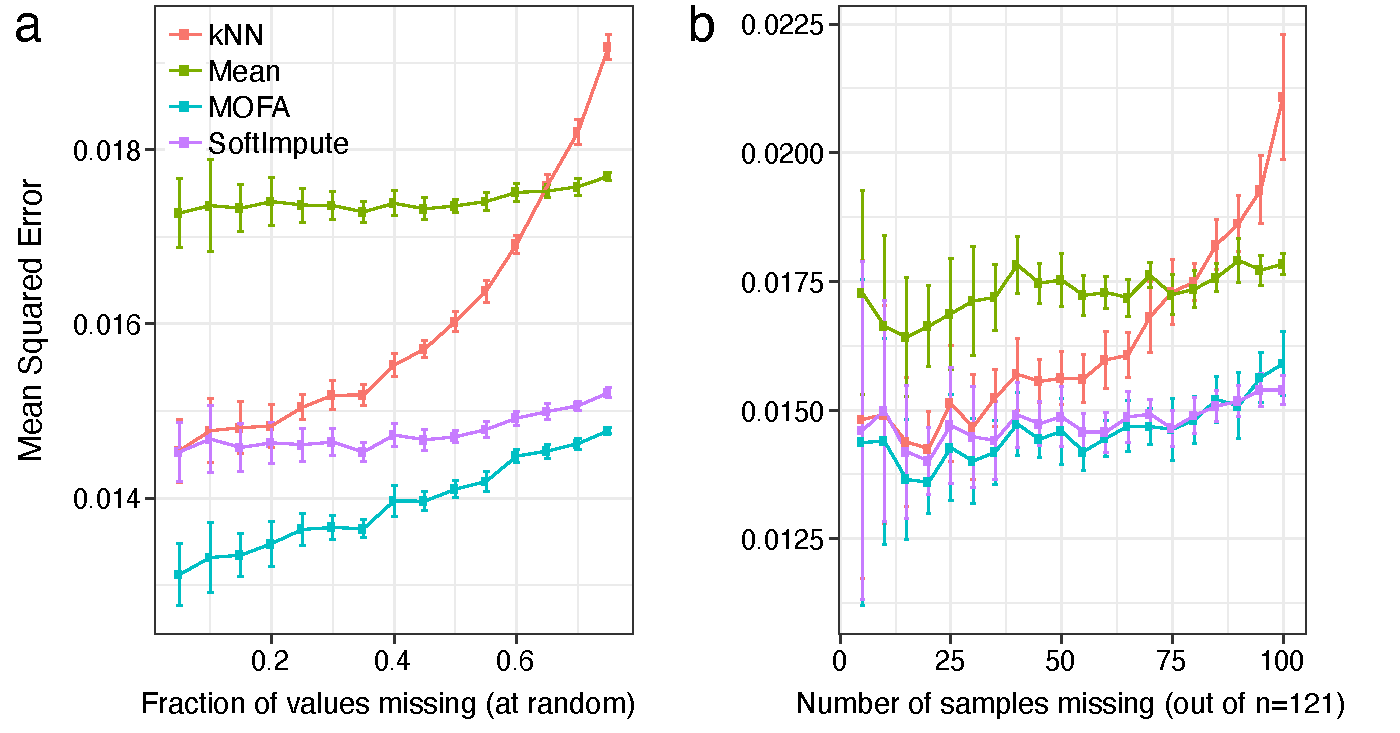
\includegraphics[width=0.9\textwidth]{MOFA_imputation}
	\caption{\textbf{Evaluation of imputation performance in the drug response assay.}\\
	The y-axis shows the mean-squared error (MSE) across 15 trials for increasing fractions of missing data (x-axis). Two experiments were considered: (a) values missing at random and (b) entire assays missing at random. Each point displays the mean across all trials and the error bars depict the corresponding standard deviations.}
	\label{fig:MOFA_imputation}
\end{figure}


\newpage

\section{Application to single-cell multi-omics} \label{section:mofa_scmt}

The emergence of single-cell multi-modal techniques has created opportunities for the development of novel computational strategies \cite{Stuart2019,Colome-Tatche2018,Chappell2018}.\\
To show case how MOFA can be used to integrate single-cell multi-omics data, we considered a simple data set that consists of 87 ESCs where RNA expression and DNA methylation were simultaneously measured using scM\&T-seq\cite{Angermueller2016}. Two populations of ESCs were profiled: the first one contains 16 cells grown in 2i media, which is known to induce a naive pluripotency state associated with genome-wide DNA hypomethylation \cite{Ficz2013}. The second population contains 71 cells grown in serum media, which contain stimuli that trigger a primed pluripotency state poised for differentiation \cite{Tosolini2016}.

\subsection{Data processing}

The RNA expression data was processed using \textit{scran}\cite{Lun2016b} to obtain log normalised counts adjusted by library size. Feature selection was performed by selecting the top 5,000 most overdispersed genes\cite{Lun2016a}. A Gaussian likelihod was used for this data modality. \\
The DNA methylation data was processed as described in Chapter 1. Briefly, for each CpG site, we calculated a binary methylation rate from the ratio of methylated read counts to total read counts. Next, CpG sites were classified by overlapping with genomic contexts, namely promoters, CpG islands and enhancers (distal H3K27ac peaks). Finally, for each annotation we selected the top 5,000 most variable CpG sites with a minimum coverage of 10\% across cells. Each of the resulting matrices was defined as a separate view for MOFA. A Bernoulli likelihod was used for this data modality.


\subsection{Model overview}

In this data set, MOFA inferred 3 factors with a minimum explained variance of 1\% (\Cref{fig:mofa_scMT}). Factor 1 captured the transition from naive to primed pluripotent states, which MOFA links to widespread coordinated changes between DNA methylation and RNA expression. Inspection of the gene weights for Factor 1 pinpoints important pluripotency markers including  \textit{Rex1/Zpf42} or \textit{Essrb} \cite{Mohammed2017}. As previously described both \textit{in vitro} \cite{Angermueller2016} and \textit{in vivo} \cite{Auclair2014}, the transition from naive to primed pluripotency state is concomitant with a genome-wide increase in DNA methylation levels. Factor 2 captured a second dimension of heterogeneity driven by the transition from a primed pluripotency state to a differentiated state, with RNA weights enriched with canonical differentiation markers including keratins and annexins \cite{Fuchs1988}.\\
Jointly, the combination of Factors 1 and 2 reconstruct the coordinated changes between the transcriptome and the epigenome along the differentiation trajectory from naive pluripotent cells to differentiated cells.

\begin{figure}[H]
	\centering 	
	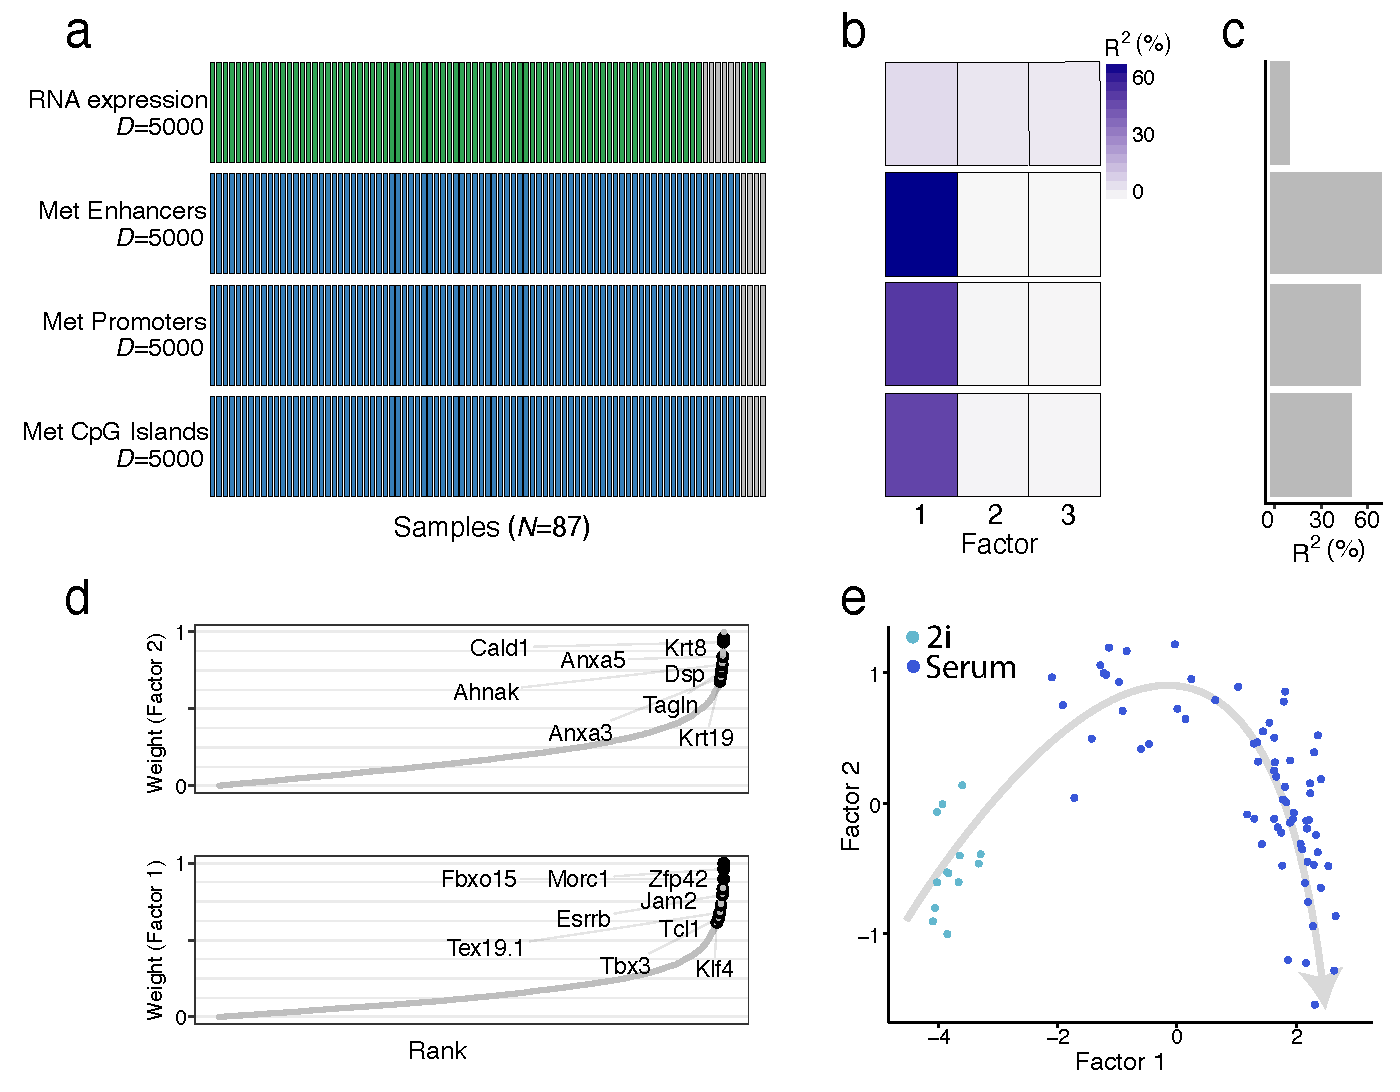
\includegraphics[width=0.9\textwidth]{MOFA_scMT}
	\caption{\textbf{MOFA recovers a differentiation process from a single-cell multi-omics data set.} \\
	(a) Overview of the data modalities. Rows indicate number of features ($D$) and columns indicate number of samples ($N$). Grey bars denote missing samples.\\
	(b) Fraction of variance explained per factor (column) and view (row).\\
	(c) Cumulative fraction of variance explained per view (across all factors).\\
	(d) mRNA weights of Factor 1 (bottom) and Factor 2 (top). The genes that are labelled are known markers of pluripotency (for Factor 1) or differentiation (for Factor 2). \\
	(e) Scatter plot of Factor 1 (x-axis) against Factor 2 (y-axis). Cells are colored based on the culture condition. Grey arrow illustrates the differentiation trajectory from a naive pluripotency state to a differentiated state. 
	}
	\label{fig:mofa_scMT}
\end{figure}

% \begin{figure}[H]
% 	\centering 	
% 	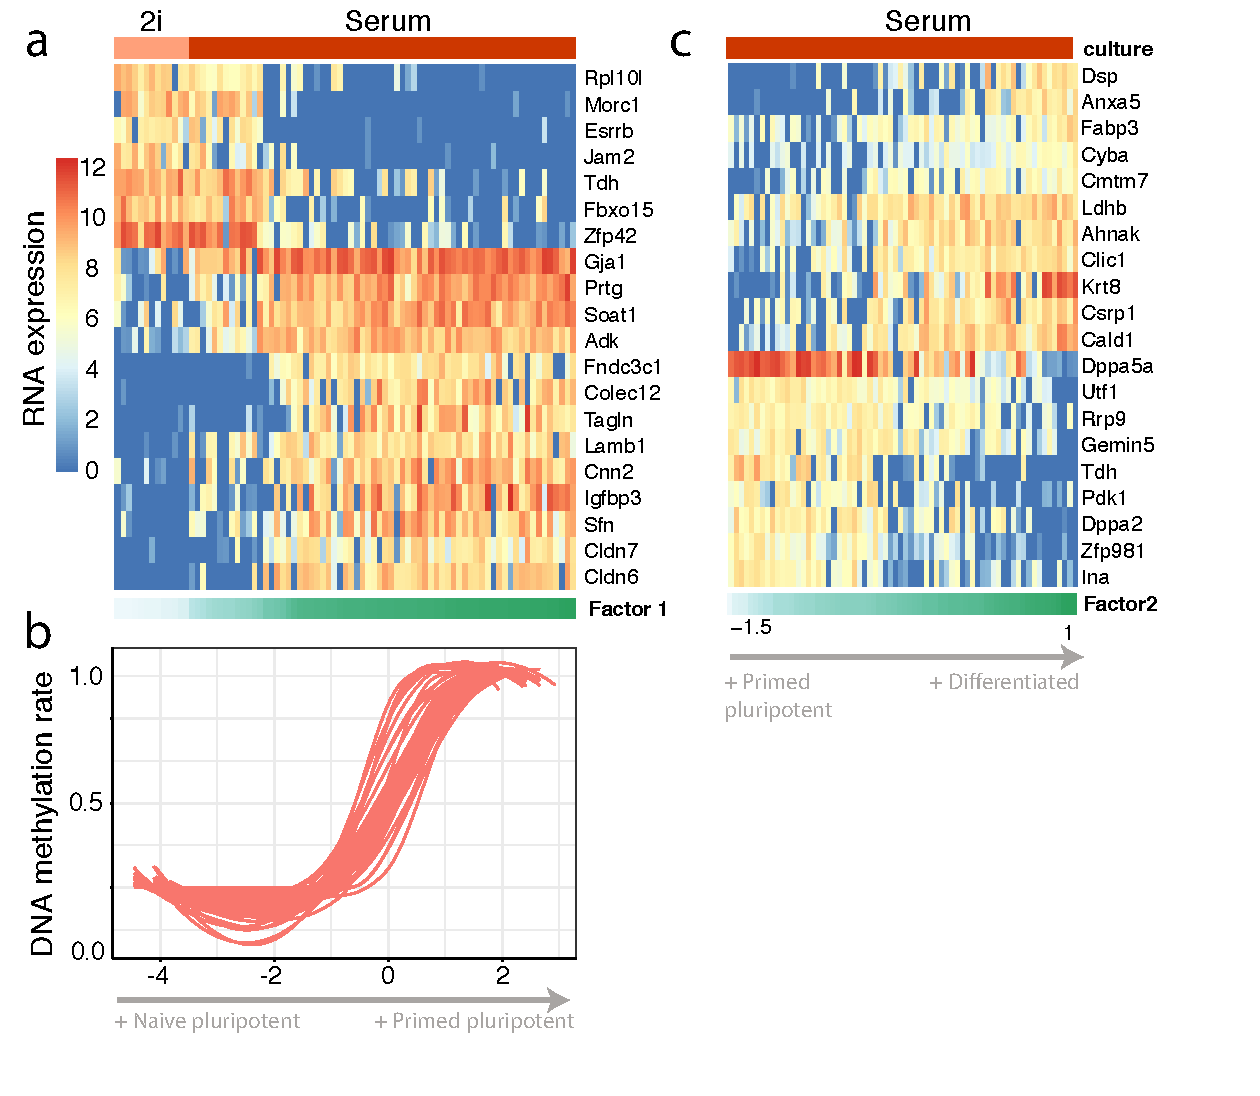
\includegraphics[width=0.8\textwidth]{MOFA_scMT2}
% 	\caption{XX}
% 	\label{fig:MOFA_scMT2}
% \end{figure}

% \subsubsection{Comparison with clustering strategies}

% To illustrate the importance of learning continuous latent spaces before clustering samples, we applied popular integrative clustering algorithms \cite{Wang2014,Shen2009,Mo2013} to the data set. As expected, two clusters can be recovered that broadly match the culture conditions. However, no trajectory is recovered, illustrating the importance of 

% \begin{figure}[H]
% 	\centering 	
% 	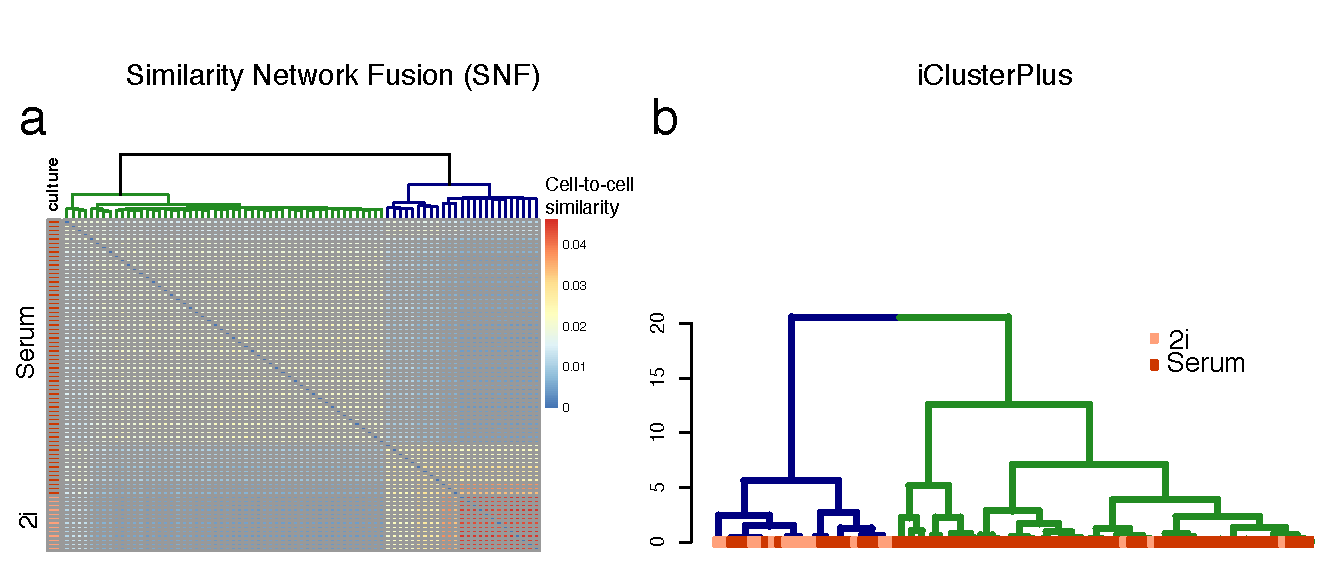
\includegraphics[width=1.0\textwidth]{MOFA_scMT_clustering}
% 	\caption{\textbf{Multi-omics clustering applied to scMT data set.}\\
% 	(a) Similarity matrix and dendogram obtained using Similarity Network Fusion\cite{Wang2014}\\
% 	(b) Dendrogram obtained using iClusterPlus\cite{Mo2013} with two clusters.
% 	}
% 	\label{fig:MOFA_scMT_clustering}
% \end{figure}

